\clearpage
\section{Architettura del sistema}
L'architettura del sistema è stata formalizzata attraverso due deployment diagram differenti: il primo, riportato in figura \ref{fig:DeplymnetDiagramNonFormale}, rappresenta il sistema tramite una notazione a stile libero, mentre il secondo, riportato in figura \ref{fig:DeplymnetDiagramFormale}, rappresenta il sistema tramite lo stile UML. In particolare, in entrambi i diagrammi è possibile identificare un pattern architetturale \textit{three layer}. All'interno del \textit{presentation layer} ci sono le applicazioni lato client che vengono utilizzate dagli attori. Nell'\textit{application layer}, invece, ci sono due macchine distinte:

\begin{itemize}
	\item su una macchina è installato un \textbf{Web Server Java}, che si occupa della gestione di richieste tramite protocollo \textit{HTTP/Rest} da parte del client;
	\item sull'altra macchina ci sono due componenti autonome, un \textbf{Data Collector} che si occupa di recuperare informazioni dai data server tramite API e le inserisce all'interno del database, ed un \textbf{Data Analyzer} che si occupa di effettuare delle analisi dei dati acquisiti con lo scopo di identificare possibili situazioni di emergenza.
\end{itemize}

Nel \textit{data layer} troviamo invece un database all'interno del quale sono inserite tutte le informazioni inerenti il sistema.

\todo{Inserire gli altri stili archietturali: Big Data Pipeline per l'applicaizone python e stile esagonale per l'implementazione delle API REST. Forse l'implementazione dello stile esagonale è da specificare dopo, come anche la Big Data Pipeline, quando li introduciamo nelle iterazioni 2 e 3. Quando mostriamo il component view.}

\begin{landscape}
	\begin{figure}[b]
		\centering
		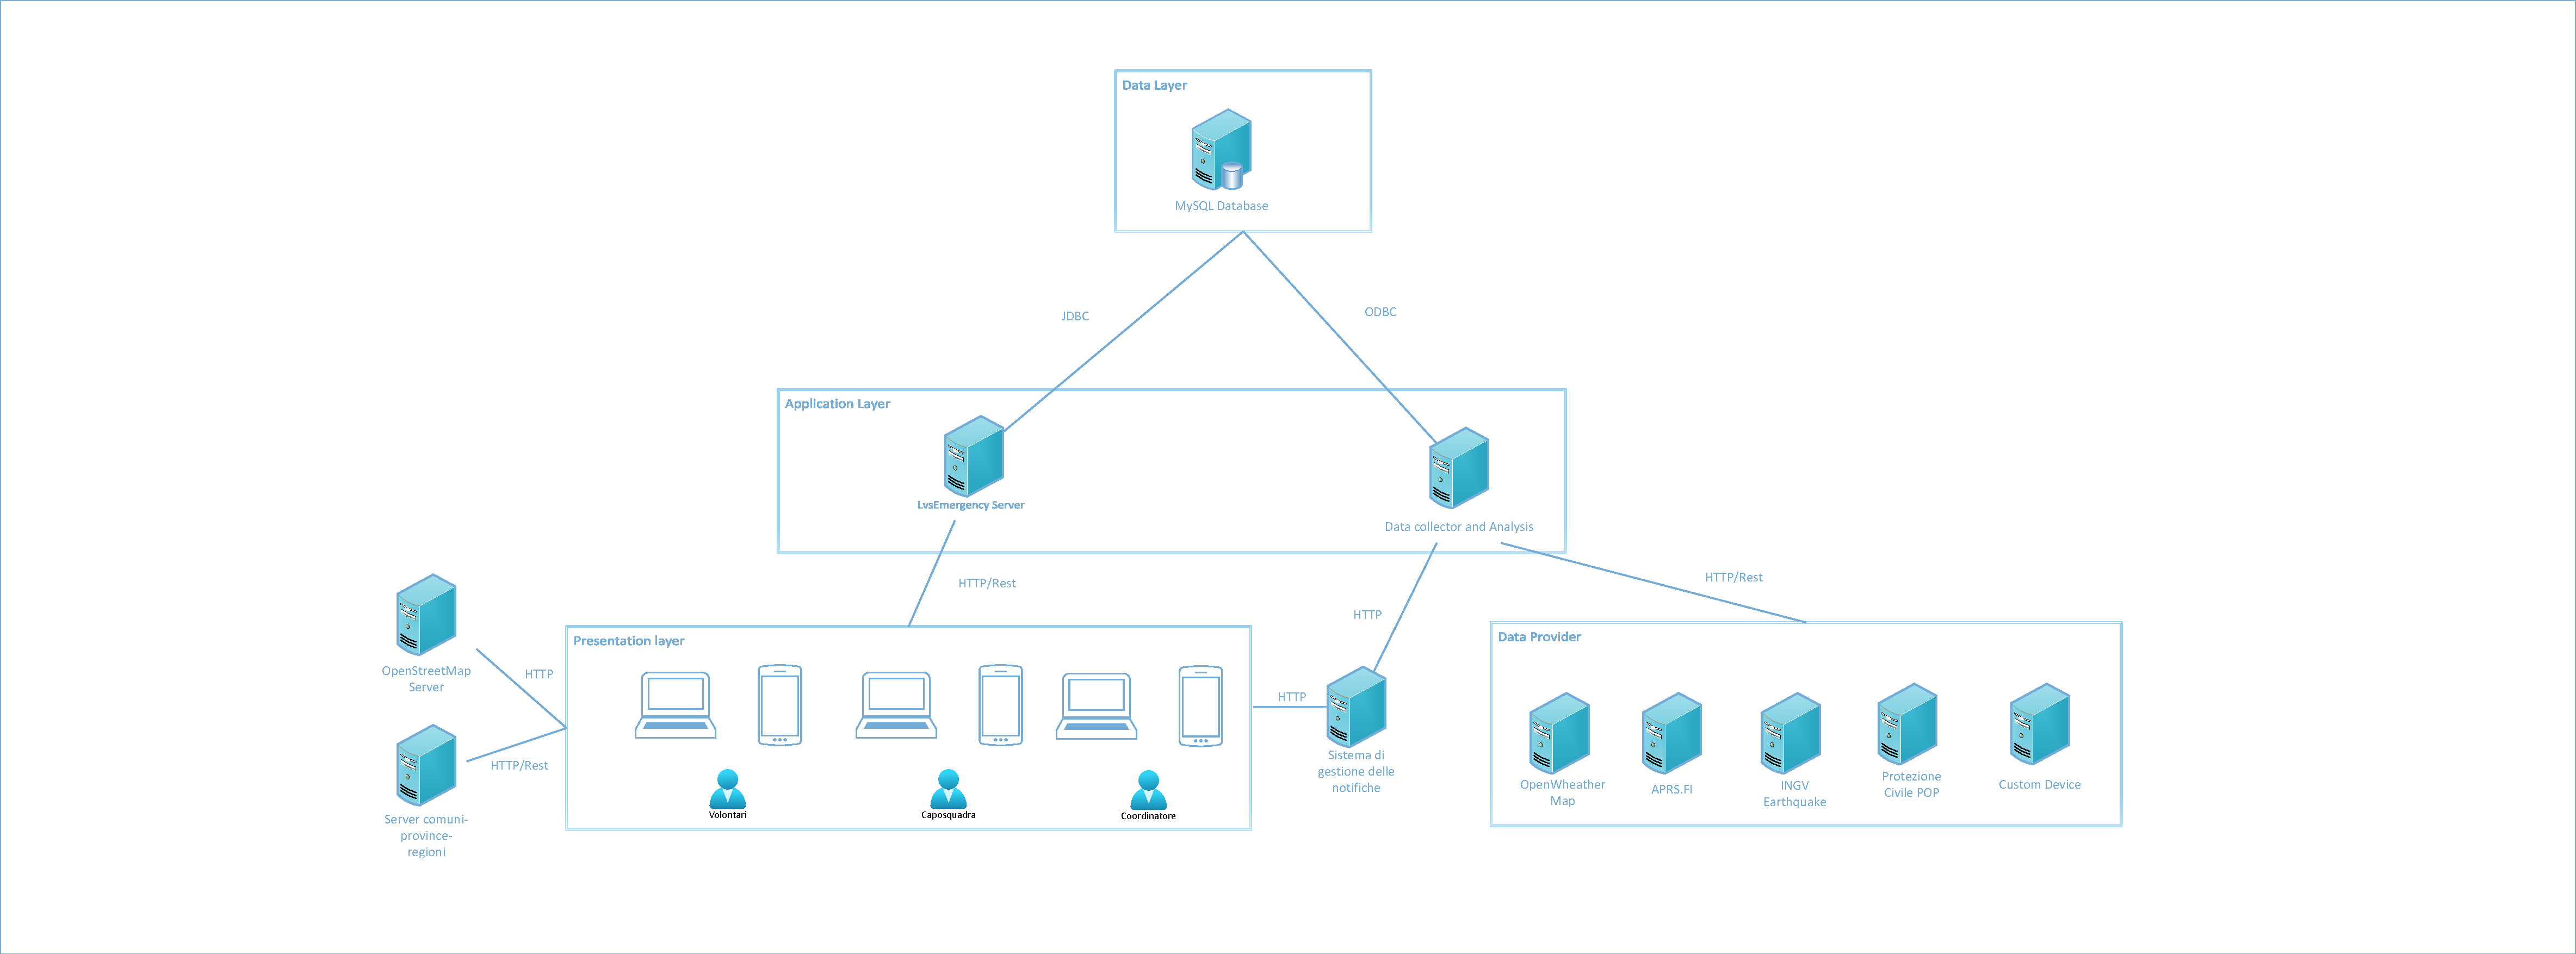
\includegraphics[width=0.9\linewidth]{./Iterazione 0/OtherFiles/DeploymentDiagramNonFormale}
		\caption{Deployment diagram in stile libero.}
		\label{fig:DeplymnetDiagramNonFormale}
	\end{figure}
\end{landscape}
\begin{landscape}
	\begin{figure}[b]
		\centering
		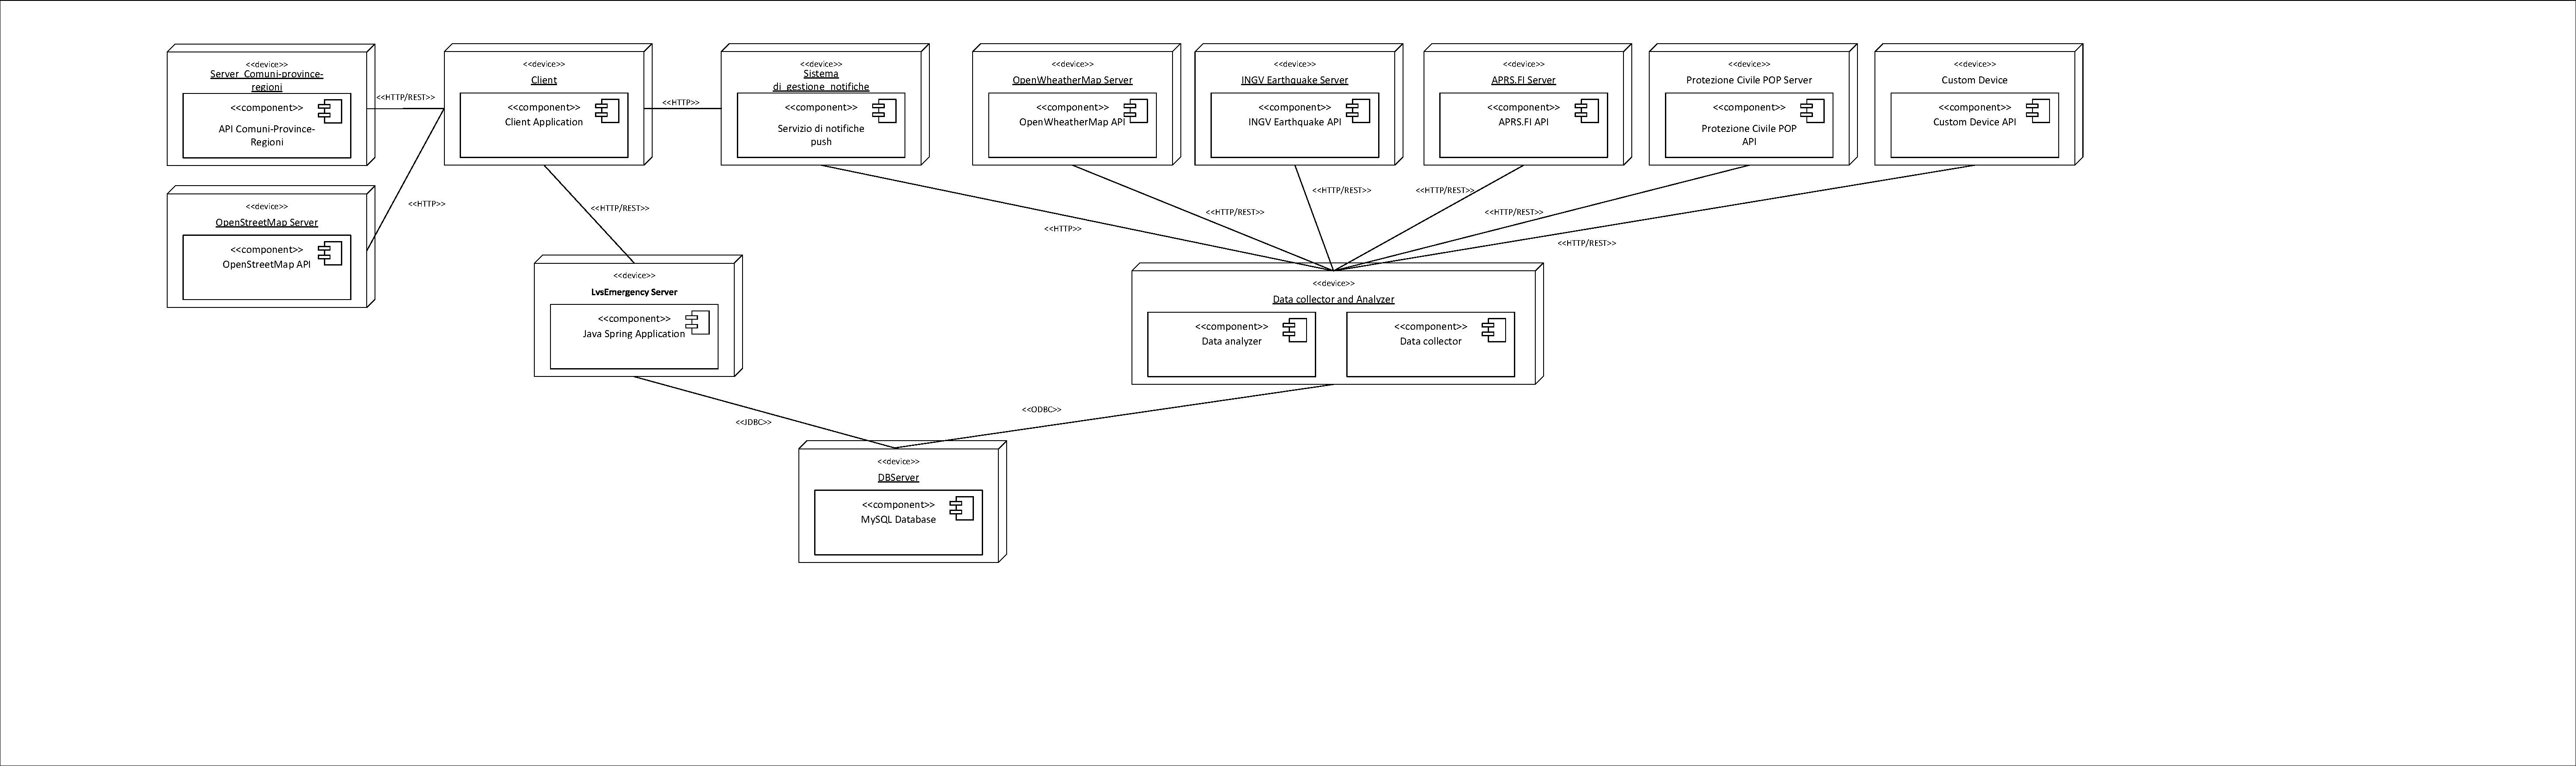
\includegraphics[width=0.9\linewidth]{./Iterazione 0/OtherFiles/DeplymentDiagramFormale}
		\caption{Deployment diagram in stile UML.}
		\label{fig:DeplymnetDiagramFormale}
	\end{figure}
\end{landscape}
